% ============================================================================
% Beamer: Image-quality inductive bias for MedVAE (Théophile's part, ~2min)
%
% USAGE: upload the figures/ folder next to this file on Overleaf (same
% relative structure), then copy-paste the frames below into your shared
% beamer deck, OR compile this file standalone (it already has a full
% preamble + \begin{document}/\end{document}).
%
% Each frame has a short "speaker note" as a LaTeX comment above it:
% delete the comments, keep the content, when copy-pasting into the
% shared deck if you don't want them cluttering the source.
% ============================================================================
\documentclass[aspectratio=169]{beamer}
\usepackage[utf8]{inputenc}
\usepackage[T1]{fontenc}
\usepackage{graphicx}
\usepackage{amsmath,amssymb}
\usepackage{booktabs}

\usetheme{Madrid}
\setbeamertemplate{navigation symbols}{}

\title{Image-quality inductive bias for MedVAE}
\subtitle{Conditioning MedVAE on an estimated quality score via FiLM}
\author{Théophile Nadiedjoa}
\institute{MedVAE: Adaptation, Fine-tuning and Analysis for Medical Imaging and Coronary Segmentation}
\date{}

\begin{document}

% ============================================================
% SLIDE 1: Motivation
% Speaker note (~15s): MedVAE applies the SAME transform to a clean or a
% noisy coronary angiography: it has no notion of "how degraded" its
% input is. Idea: estimate a quality score c in [0,1] and condition the
% VAE on it via FiLM, so it can adapt its behaviour to the actual input
% quality. Three independent ways to compute c are compared in parallel.
% ============================================================
\begin{frame}{Motivation}
  \begin{itemize}
    \item MedVAE applies the \textbf{same transform} to a clean or a heavily
      degraded coronary angiography: no notion of \emph{how degraded} the
      input is.
    \item \textbf{Hypothesis:} conditioning MedVAE on a quality score
      $c \in [0,1]$, injected via FiLM, should let it adapt to the
      degradation level actually present.
    \item Three independent ways to compute $c$ (A: weighted, B: PCA,
      C: learned) $\rightarrow$ run the \emph{same} pipeline three times.
  \end{itemize}
\end{frame}

% ============================================================
% SLIDE 2: Quality score construction pipeline
% Speaker note (~20s): per-patch IQA metrics (Laplacian, contrast,
% entropy, directional Tenengrad) + ResNet-18 features, merged into a
% single score c by 3 independent methods: weighted combination, PCA,
% and an MLP trained on synthetic degradations.
% ============================================================
\begin{frame}{Building the quality score $c$}
  \begin{center}
    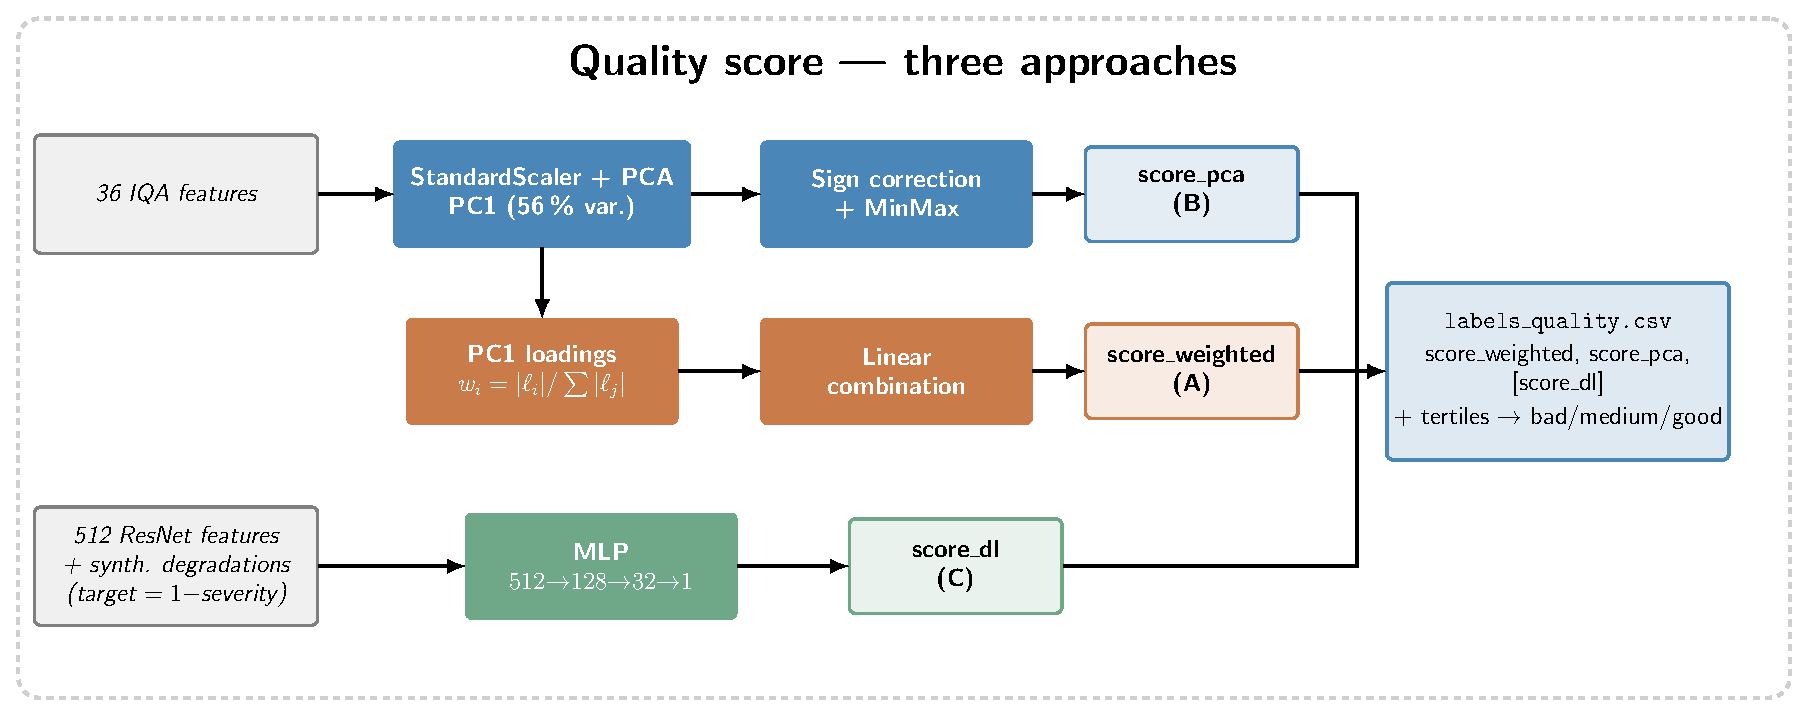
\includegraphics[width=0.95\textwidth]{figures/pipeline_B_score.pdf}
  \end{center}
\end{frame}

% ============================================================
% SLIDE 3: Qualitative sanity check on the score
% Speaker note (~10s): sorting real ARCADE images by increasing score
% gives a visual confirmation: noisy/blurry images on the left, sharp
% contrasted vascular trees on the right.
% ============================================================
\begin{frame}{Does the score make clinical sense?}
  \begin{center}
    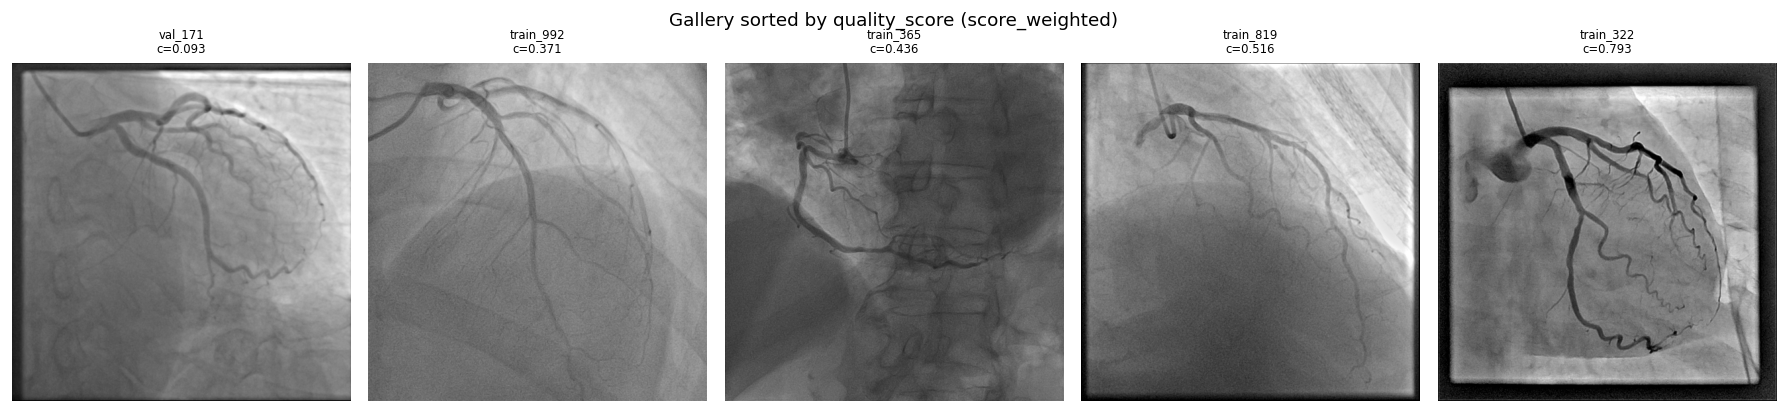
\includegraphics[width=\textwidth]{figures/result_gallery_score.png}
  \end{center}
  \begin{center}
    \footnotesize ARCADE images sorted by increasing score $c$ (approach A).
  \end{center}
\end{frame}

% ============================================================
% SLIDE 4: FiLM conditioning + training pipeline
% Speaker note (~20s): inject c via FiLM on all 19 ResnetBlocks
% (encoder+bottleneck+decoder), zero-init so the conditioned model starts
% identical to MedVAE. Two-phase training (FiLM warm-up, then full
% fine-tune), with a strictly identical unconditioned baseline trained
% on the same budget for a fair comparison.
% ============================================================
\begin{frame}{FiLM conditioning \& training}
  \begin{center}
    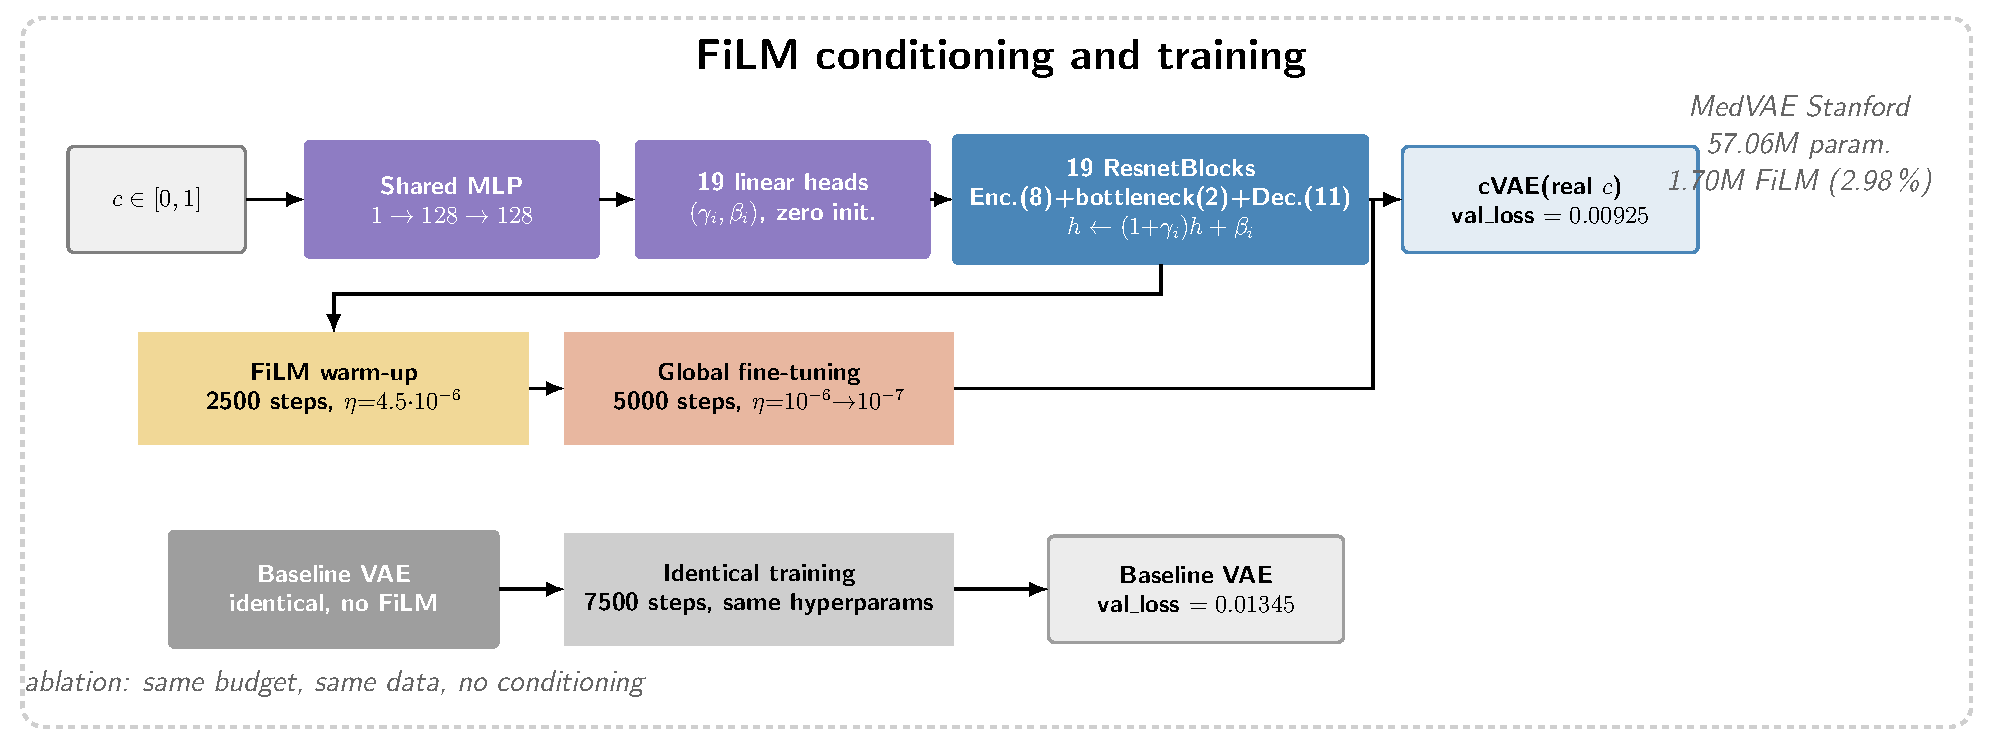
\includegraphics[width=0.95\textwidth]{figures/pipeline_C_film.pdf}
  \end{center}
\end{frame}

% ============================================================
% SLIDE 5: Main result: baseline beats the conditioned cVAE
% Speaker note (~25s): counter-intuitive result. Measured properly on an
% independent test set, in pixel space (not the internal training loss,
% which was misleading): the UNCONDITIONED baseline reconstructs better
% than the cVAE, on all 3 score approaches and all 4 metrics, no
% exception. Boxplots: PSNR distribution (classic & vessel-masked) is
% systematically shifted down for the cVAE, in every quality class.
% ============================================================
\begin{frame}{Result: conditioning hurts reconstruction}
  \begin{center}
    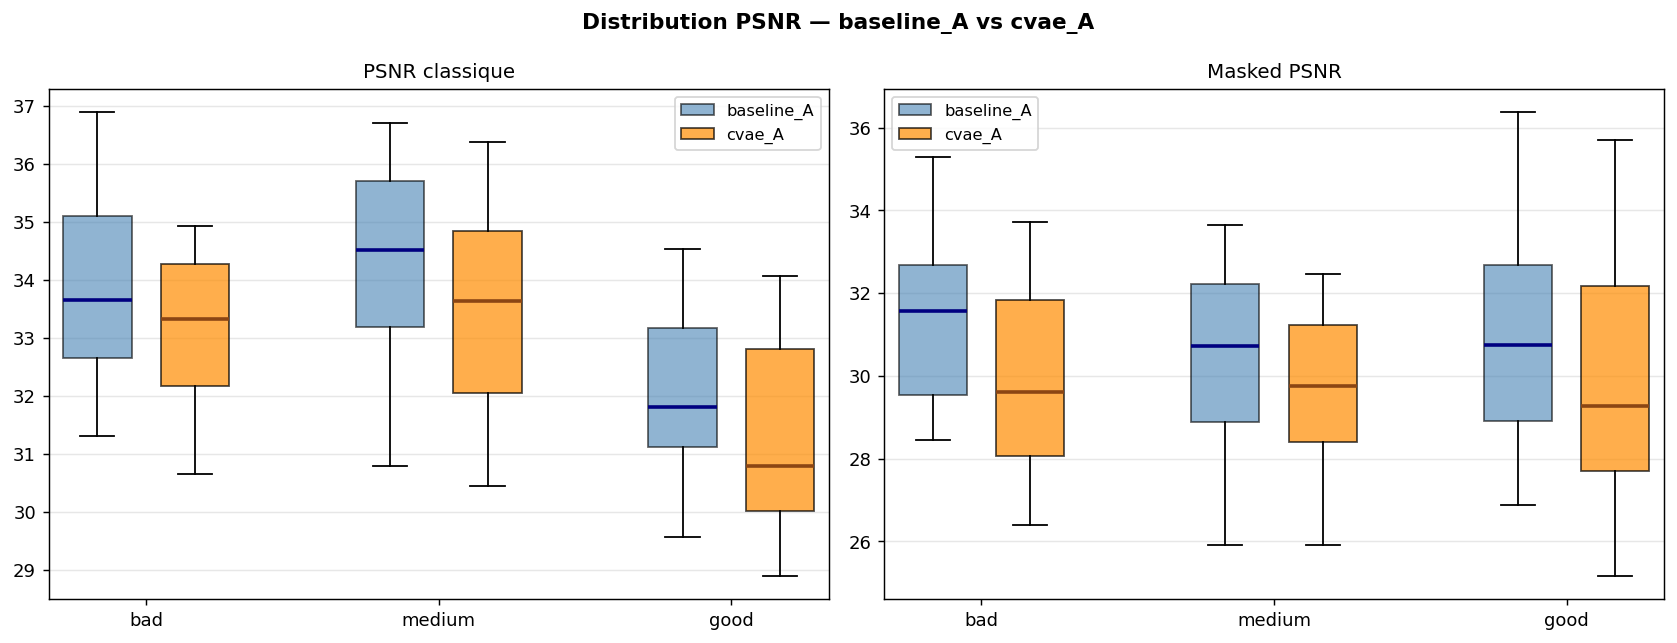
\includegraphics[height=0.62\textheight]{figures/bonus_boxplots_psnr.png}
  \end{center}
  \footnotesize
  \begin{itemize}
    \item Baseline $>$ cVAE on \textbf{all 3 approaches} $\times$
      \textbf{all 4 metrics} (MSE, SSIM, PSNR, HaarPSI), even masked
  \end{itemize}
\end{frame}

% ============================================================
% SLIDE 6: Ablation: is c actually used?
% Speaker note (~25s): train a second cVAE with a CONSTANT c=0.5 instead
% of the real score. Only approach C (the learned score) shows the
% network truly exploits c: on all 4 metrics. So the degradation isn't
% due to an inert mechanism: it's a genuine architecture trade-off, FiLM
% perturbs the decoder's optimisation more than it helps, within this
% training budget.
% ============================================================
\begin{frame}{Ablation: does the network actually use $c$?}
  \begin{center}
    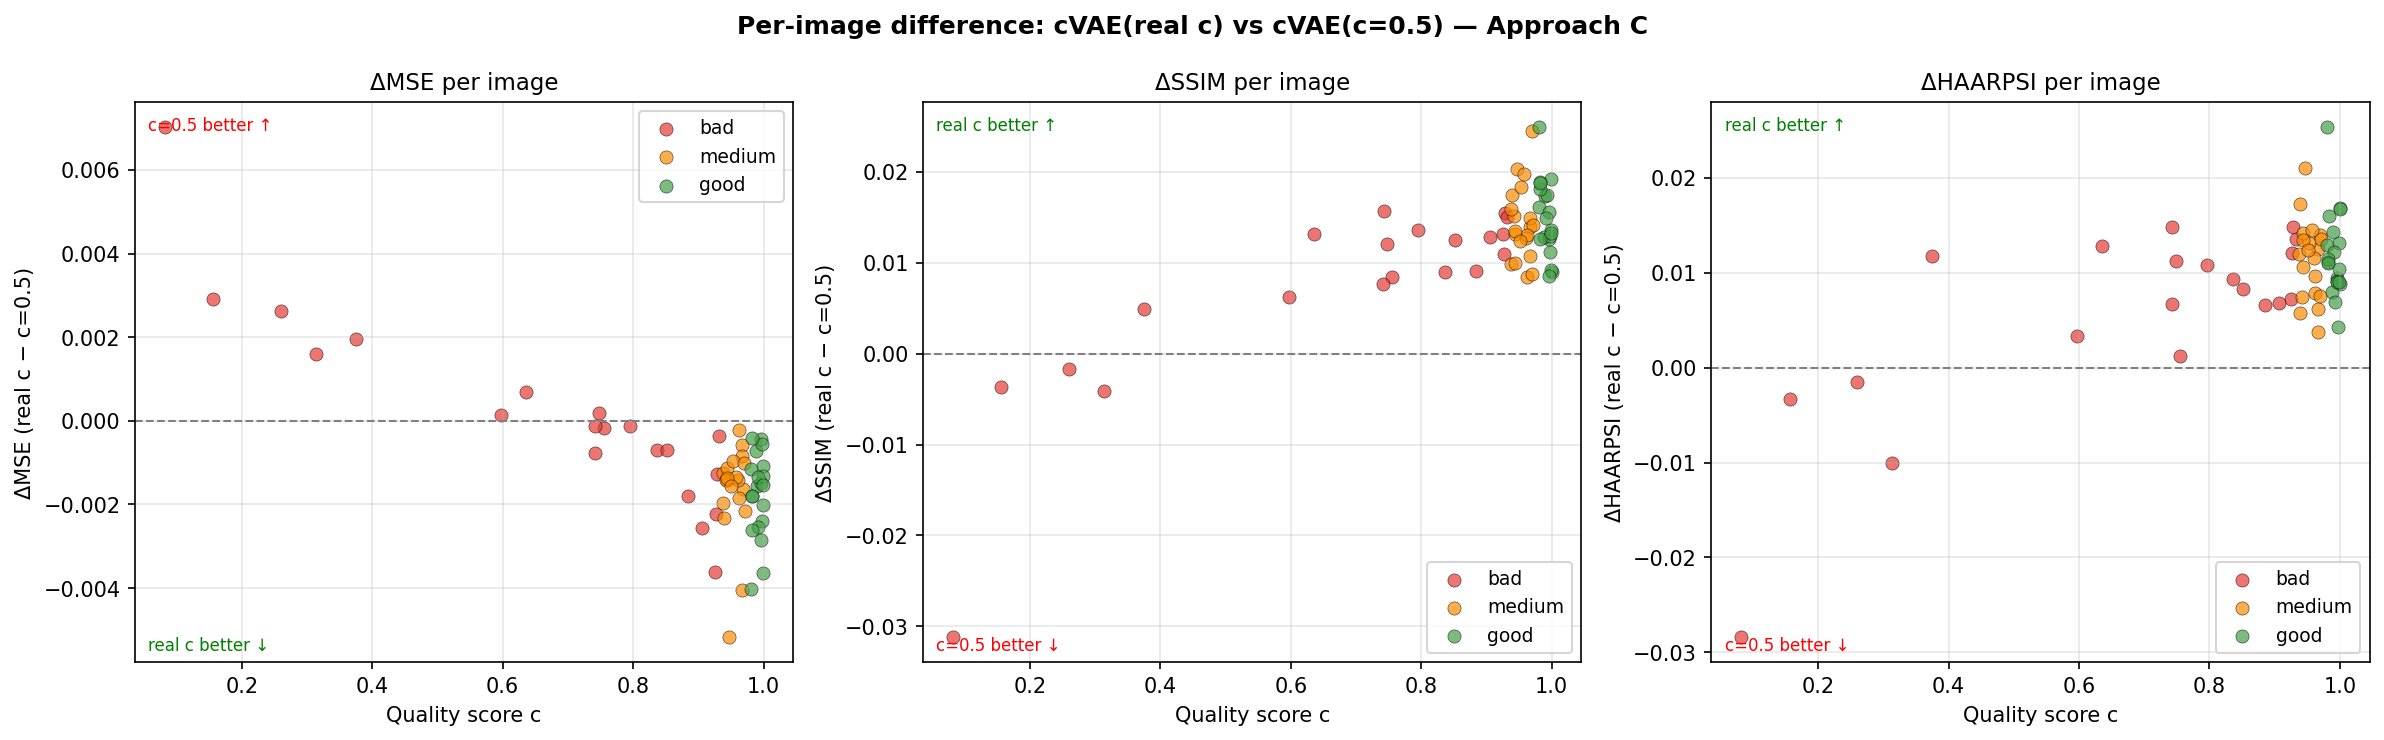
\includegraphics[width=0.85\textwidth]{figures/result_delta_ablation.png}
  \end{center}
  \begin{center}
    \footnotesize Real $c$ vs.\ constant $c{=}0.5$ (approach C): gap grows
    with image quality: the network's response genuinely depends on $c$.
  \end{center}
\end{frame}

\end{document}
